\section{Quantum gates}

After recalling the postulates of QM we want to focus a little on the second one and understanding how we can manipulate the states of qubits using it. In particular, the second postulate tells us that the evolution of a state in time is described by a unitary operator $\mathcal{U}$. Normally that operator should have infinite dimensions, nevertheless the qubits posses a finite dimensional Hilbert space meaning that also the operators inside it can be associated to finite matrices. To understand this we can take a system composed by $N$ qubits, so that $\dim\mathcal{H} = 2^N$, the operator could then be described as follows
\begin{align}
    &\mathcal{U}: \mathbb{C}^{2N} \to \mathbb{C}^{2N}, &\mathcal{U} = \begin{pmatrix}
        a_{11} & \cdots & a_{2^{N}1}\\
        \vdots & \ddots & \vdots\\
        a_{12^N} & \cdots & a_{2^N2^N}
    \end{pmatrix}.
\end{align}
This representation is incredibly useful on a mathematical level, in fact manipulating a simple qubit state will become as doing a matrix multiplication. In particular, we know that the state of a qubit can be written generally as $\ket{\psi} = a\ket{0} + b\ket{1} = (a, b)$, so applying a generic state manipulation $\mathcal{U}$ will simply mean doing the following
\begin{equation}
    \label{eq:singleQuOp}
    \mathcal{U}\ket{\psi} = \begin{pmatrix}
        A & B\\
        C & D
    \end{pmatrix}\begin{pmatrix}
        a\\
        b
    \end{pmatrix} = 
    \begin{pmatrix}
        Aa + Bb\\
        Ca + Db
    \end{pmatrix} = \ket{\psi'}.
\end{equation}
This matrix operations are called \textbf{quantum gates}, and we want to try to unveil some possible interesting forms that they can have starting to understand how effectively a so-called \textbf{quantum circuits} works. In fact, a quantum circuits is non-other than a series of quantum gates acting on the available qubits in order to obtain a specific state in the end, as depicted in \figref{fig:FirstQC}.
\begin{figure}[b]
    \centering
    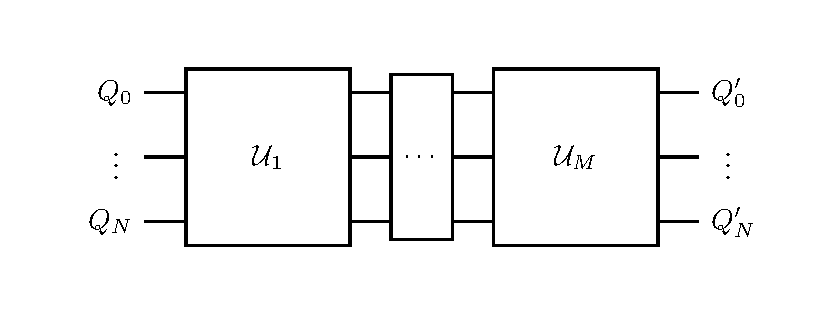
\includegraphics[width=0.91\textwidth]{Immagini/FirstQC.pdf}
    \caption{
        Sample image of a general quantum circuits where all the manipulations on the qubits are done using quantum gates, matrices, represented as blocks. 
    }
    \label{fig:FirstQC}
\end{figure}

Thus, what we want to do now is look deeper in the form that those gates can have, and try to identify some important operations that will follow us during the whole course. Therefore, I suggest to the reader (especially my future self) to look into them and try getting attune to their form and their actions on the qubits.

\subsection{Single qubit gates}

The first type of gates that we want to analyze are the one that acts a single qubits, which are also the simplest ones. As we have pointed out previously an operation of this type can be written as a matrix like in \eqref{eq:singleQuOp}. In particular, it's easy to understand that every $2\times 2$ matrix that is unitary satisfy the second postulate being a valid quantum gate for the manipulation of a qubit state. That let us have an infinite amount of possibilities for the operations that we can do on a single unit of information, setting another difference with the classical bits. In fact, a normal bit could be manipulated through the application of the identity operation, leaving as it is, or the NOT one, changing its state. So, not only the qubits allow for an infinite number of possible states to be represented using superposition, but also allow for an infinite number of operations to be done on it showing a clear superiority.

This simple observation has already shown to us that we have a lot of room in which we can move in order to work with qubit, and what we need to do now is to point out the most significant and important operations that are present inside this really large space. The first, thing that is important to point out is that we know how to generate every $2\times 2$ unitary matrix using four of them. Thus, mathematic has already given us a way to write down all the possible gates using a simple universal relation.
\thm{Universal single gate}
{
    Every quantum gate $\mathcal{U}$ can be associated to a rotation of the state on the Bloch sphere, and therefore can be written as
    \begin{equation}
        \mathcal{U} = e^{i\lambda\mathbb{1}}\exp\left( ia\vb{n}\vdot\vb*{\sigma} \right),
    \end{equation}
    where $\lambda, \alpha\in \mathbb{R}$, $\mathbb{1}$ is the identity matrix, $\vb{n}$ is an appropriate unitary vector, and $\vb*{\sigma}$ is a vector containing the three Pauli matrices.
    \begin{align}
        X = \mqty(\pmat{1}), \hspace{2cm} Y = \mqty(\pmat{2}), \hspace{2cm} Z = \mqty(\pmat{3}). 
    \end{align}
}
\noindent
This theorem tells us that only $4$ parameters are needed in order to define every possible gates, in fact the parameter $a$ is not really needed can be associated to the velocity of the rotation not really on the rotation itself. Therefore, we know how to write every possible operation, still the one that are interesting to us are limited, and so we will report them briefly discussing the form and the action of those specific gates.

\paragraph{NOT.} The NOT operation is the equivalent of the one in the classical case, meaning that the effect is the one of negating the current state. That can be easily done by recalling that the $0$ and $1$ of our quantum logic are the state $\ket{0}$ and $\ket{1}$, leading us to the possibility of constructing the truth table and matrix associated to this operation.

\begin{minipage}{0.45\textwidth}
    \centering
    \begin{tabular}{c|c}
        \textbf{IN} & \textbf{OUT}\\
        \midrule
        $\ket{0}$ & $\ket{1}$\\
        $\ket{1}$ & $\ket{0}$
    \end{tabular}
\end{minipage}
\begin{minipage}{0.45\textwidth}
    \centering
    \begin{equation}
        \text{NOT} = \scalebox{1.5}{$\begin{pmatrix}
            0 & 1\\
            1 & 0
        \end{pmatrix}$}
    \end{equation}.
\end{minipage}

\noindent
One can also notice that the final matrix obtained is exactly the $X$ Pauli matrix, with assure to us that is unitary since every one of them has the property $X^2 = Y^2 = Z^2 = \mathbb{1}$. This matrix is, in fact, drawn as $\bigoplus$ symbol inside circuits to recall that the $X$ matrix is getting used on a certain qubit.

\paragraph{Hadamart.} This is the first real quantum gate that was thought of, the idea is the one of creating superpositions of the normal states. This can be done really easily since the gate that we are interested in, and it's truth table, is

\begin{minipage}{0.45\textwidth}
    \centering
    \begin{tabular}{c|c}
        \textbf{IN} & \textbf{OUT}\\
        \midrule
        $\ket{0}$ & $\ket{+}$\\
        $\ket{1}$ & $\ket{-}$
    \end{tabular}
\end{minipage}
\begin{minipage}{0.45\textwidth}
    \centering
    \begin{equation}
        H = \scalebox{1.5}{$\frac{1}{\sqrt{2}}\begin{pmatrix}
            1 & 1\\
            1 & -1
        \end{pmatrix}$}
    \end{equation}.
\end{minipage}

\noindent
Where we shall recall how $\ket{\pm} = (\ket{0} \pm \ket{1})/\sqrt{2}$ are interesting states that forms the eigenvectors of the $X$ Pauli matrix, basically being the states in the $x$ direction on the Bloch sphere while the computational base is on the $z$ one. This gate has also really important properties that can be interesting such as
\begin{equation}
    H^2 = \mathbb{1}, \hspace{2cm} H^\dagger = H = H^{-1}, \hspace{2cm} HZH = X.
\end{equation}

\paragraph{Phase.} This is another type of gate that wants to do a purely quantum operation, that is the one of adding a phase shift to the two components of the state. Basically we want a gate that starting from a state $\ket{\psi} = a\ket{0} + b\ket{1}$ is able to add a phase shift to the two bases that can be used to enhance interference effects. The idea is so the follwing
\begin{align}
    &\Phi(\theta)\ket{\psi} = a\ket{0} + be^{i\theta}\ket{1}, & \Phi(\theta) = \begin{pmatrix}
        1 & 0\\
        0 & e^{i\theta}
    \end{pmatrix}.
\end{align} 
These types of gates can be used in a lot of situations since phase shift are really common inside quantum mechanical application, and some of them are most commonly used than the others and so a specific name was given to them
\begin{equation}
    \Phi(\pi/2) = \begin{pmatrix}
        1 & 0\\
        0 & i
    \end{pmatrix} = S, \hspace{2cm}
    \Phi(\pi/4) = \begin{pmatrix}
        1 & 0\\
        0 & \frac{1+i}{\sqrt{2}}
    \end{pmatrix} = T, \hspace{2cm}
    T^2 = S.
\end{equation}

\nt
{
    I want to stress out how the idea of the qubit is basically creating a new type of logic. In the classical computers the boolean logic was the only possible thing with the bits that could be only 0 and 1 along with two possible operations: identity or NOT. Now, the qubit can have infinite states and infinite operations can be done on it having so an incredible much richer logic that allow things obviously impossible before. An example of it is the $\sqrt{\text{NOT}}$ operation which was demonstrated impossible to define since no operation applied to times could bring to the NOT one, even inside the context of fuzzy logic. In quantum logic we can do it simply by taking the square root of the Pauli matrix
    \begin{equation}
        \sqrt{X} = \frac{1}{2}\begin{pmatrix}
            1+i & 1-i\\
            1-i & 1+i
        \end{pmatrix}.
    \end{equation}
}

\subsection{Two qubits gates}

The next step is adding a second qubit to our system and see how the possible gates changes. On a mathematical level the answer is really simple since we are simply modifying $\mathcal{H}$ to have two more dimensions, having so that now $\mathcal{U}: \mathbb{C}^{4}\to\mathbb{C}^4$ being represented by a $4\times 4$ unitary matrix. Thus, the possibilities for the usable gates have increased respect to the single qubit once. Nevertheless, also in this case we want to make some order and explicitly write down the ones that are used the most and that we will see more frequently.

\paragraph{Control.} The control gates, in reality, are a class of two qubits gates that one of the two as the control one, not being modified, and perform operations on the other. To understand the concept we can have a look at the most important control gate that is the \textbf{CNOT}. The latter is a gate that takes two qubits and: when the control one is $\ket{0}$ then nothing is done, if the control is $\ket{1}$ then the NOT is performed on the other qubit. At first this gate may seem complicated to realize, but that would be a wrong assumption since both the truth table and matrix are simple as

\begin{minipage}{0.45\textwidth}
    \centering
    \begin{tabular}{c|c}
        \textbf{IN} & \textbf{OUT}\\
        \midrule
        $\ket{00}$ & $\ket{00}$\\
        $\ket{01}$ & $\ket{01}$\\
        $\ket{10}$ & $\ket{11}$\\
        $\ket{11}$ & $\ket{10}$
    \end{tabular}
\end{minipage}
\begin{minipage}{0.45\textwidth}
    \centering
    \begin{displaymath}
        \text{CNOT} = \begin{pmatrix}
            \begin{pmatrix}
                1 & 0\\
                0 & 1
            \end{pmatrix} &  \begin{matrix}
                0 & 0\\
                0 & 0
            \end{matrix}\\
            \begin{matrix}
                0 & 0\\
                0 & 0
            \end{matrix} & \begin{pmatrix}
                0 & 1\\
                1 & 0
            \end{pmatrix}
        \end{pmatrix} = \begin{pmatrix}
            \mathbb{1} & \mathbb{0}\\
            \mathbb{0} & X
        \end{pmatrix}.
    \end{displaymath}.
\end{minipage}

\noindent
Where we can see how the total matrix is formed by the use of two known single qubit gates on the diagonal, creating the quantum version of the NOR opeartion in boolean logic. This form, with two gates on the diagonal, allow for a big flexibility inside this category of matrices, in particular it's easy to understand that one can create the C-version of every single qubit operator by simply defining it as

\begin{minipage}{0.45\textwidth}
    \centering
    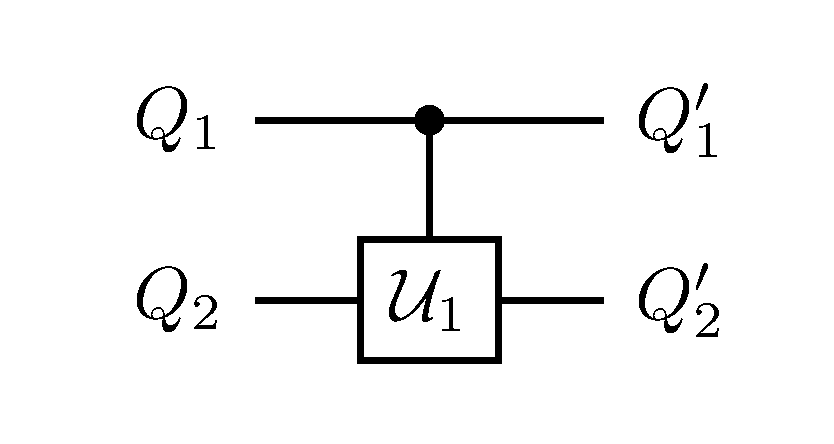
\includegraphics[width=0.8\textwidth]{Immagini/ContrU.pdf}
\end{minipage}
\hspace{-1cm}
\begin{minipage}{0.45\textwidth}
    \begin{equation}
        \text{C}\mathcal{U} = \begin{pmatrix}
            \mathbb{1} & \mathbb{0}\\
            \mathbb{0} & \mathcal{U}
        \end{pmatrix}.
    \end{equation}
\end{minipage}

\noindent
Where, in the graphical representation the dot describe the control qubit.

\paragraph{Swap.} This gate is in reality a simple circuits constructed using three CNOT gates in order, and the reason of the name can be easily seen by the truth table.

\begin{minipage}{0.45\textwidth}
    \centering
    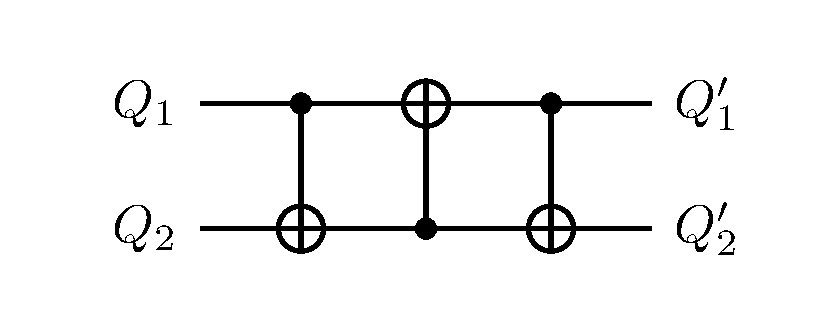
\includegraphics[width=0.9\textwidth]{Immagini/SwapCirc.pdf}
\end{minipage}
\hspace{-1cm}
\begin{minipage}{0.45\textwidth}
    \centering
    \begin{tabular}{c|c}
        \textbf{IN} & \textbf{OUT}\\
        \midrule
        $\ket{00}$ & $\ket{00}$\\
        $\ket{01}$ & $\ket{10}$\\
        $\ket{10}$ & $\ket{01}$\\
        $\ket{11}$ & $\ket{11}$
    \end{tabular}
\end{minipage}
\vspace{0.3cm}

\noindent
Thus, one can see that the effect is literally the one of swapping the states of the qubit. This is a simple and clever operation that can be written in a simple matrix form thanks to the fact that we know the matrix describing the gate of the circuit of which is formed. Therefore, we can write down the final gate by simply matrix multiplying the gates of which is composed in the right order and then having the following one described by its own simbol

\begin{minipage}{0.45\textwidth}
    \centering
    \includegraphics[width=0.8\textwidth]{Immagini/Swapsim.pdf}
\end{minipage}
\hspace{-1cm}
\begin{minipage}{0.45\textwidth}
    \begin{equation}
        \text{SWAP} = \begin{pmatrix}
            1 & 0 & 0 & 0 \\
            0 & 0 & 1 & 0 \\
            0 & 1 & 0 & 0 \\
            0 & 0 & 0 & 1 \\
        \end{pmatrix}.
    \end{equation}
\end{minipage}

\paragraph{Bell.} This is a simple circuit that nevertheless is really important since allow for the creation of particular states of major interest in physics, the Bell's states. The latter are four quantum mechanical states defined as follows
\begin{align}
    &\psi^{\pm} = \frac{1}{\sqrt{2}}\left( \ket{00} \pm \ket{11} \right), &\phi^{\pm} = \frac{1}{\sqrt{2}}\left( \ket{01} \pm \ket{10} \right).
\end{align}
They are mostly important in the theoretical study of spin states, but they appear also in other areas of QM. Thus, we want to describe a circuit that is able to prepare the system in those states and the way in which this can be done is the following

\begin{minipage}{0.45\textwidth}
    \centering
    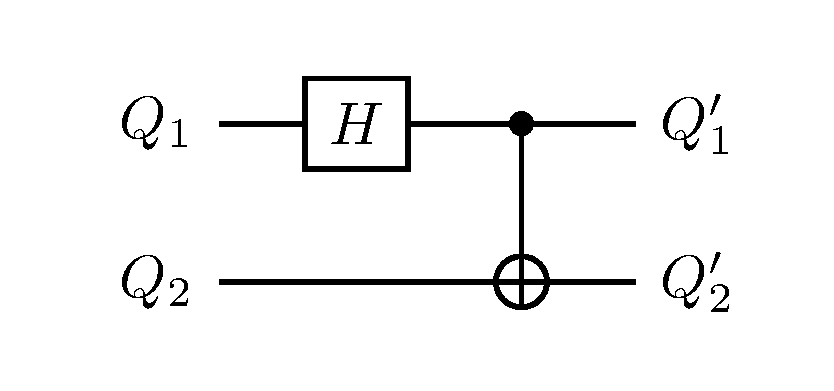
\includegraphics[width=\textwidth]{Immagini/BellCirc.pdf}
\end{minipage}
\hspace{-1cm}
\begin{minipage}{0.45\textwidth}
    \centering
    \begin{tabular}{c|c}
        \textbf{IN} & \textbf{OUT}\\
        \midrule
        $\ket{00}$ & $\psi^+$\\
        $\ket{01}$ & $\phi^+$\\
        $\ket{10}$ & $\psi^-$\\
        $\ket{11}$ & $\phi^-$
    \end{tabular}
\end{minipage}
\vspace{0.3cm}

\noindent
Basically, based on the initial state of the system we are able to generate one of the four Bell state and then study their behavior in specific circuits. 

\ex{Circuit solving}
{
    As a scrupulous, I want to see the computation of the Bell's gate output for the case $\ket{10}$ just to show the reader how effectively solve the circuit. At first the Hadamart gate is used on the first qubit
    \begin{equation}
        H\ket{1}\ket{0} = \frac{1}{\sqrt[]{2}}\left( \ket{0}\ket{0} - \ket{1}\ket{0} \right) = \frac{1}{\sqrt[]{2}}\left( \ket{00} - \ket{10} \right),
    \end{equation}
    then the CNOT operation is applied using the first qubit as control, having the final result
    \begin{equation}
        \psi^+ = \frac{1}{\sqrt{2}} = \left( \ket{00} - \ket{11} \right)
    \end{equation}
}

\subsection{N qubits gates}

We can now step into assuming to have a general number of qubits to work with and see how some general gates can effectively be created also in this case, in particular two main types of gates play a huge role in the whole theory of quantum computers.

\paragraph{Toffoli.} This is a specific 3-qubit gate that has the aim of making a control NOT gate using two different controls. Basically, having two controls the idea is to apply the NOT to the target if and only if both the two controls are in state $\ket{1}$. For this reason the gate is also called CCNOT and has the following matrix and circuit representation

\begin{minipage}{0.45\textwidth}
    \centering
    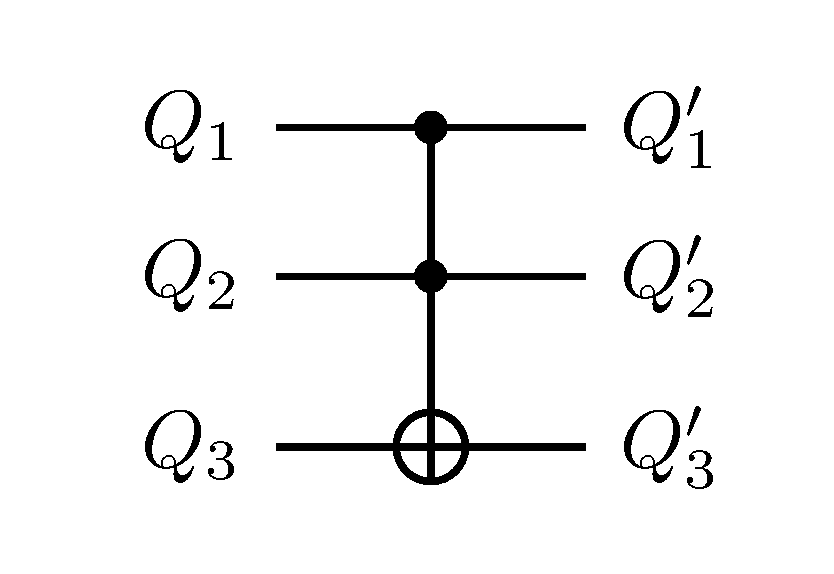
\includegraphics[width=\textwidth]{Immagini/Toffoli.pdf}
\end{minipage}
\begin{minipage}{0.45\textwidth}
    \begin{displaymath}
        \text{CCNOT} = \begin{pmatrix}
            1 & 0 & 0 & 0 & 0 & 0 & 0 & 0\\
            0 & 1 & 0 & 0 & 0 & 0 & 0 & 0\\
            0 & 0 & 1 & 0 & 0 & 0 & 0 & 0\\
            0 & 0 & 0 & 1 & 0 & 0 & 0 & 0\\
            0 & 0 & 0 & 0 & 1 & 0 & 0 & 0\\
            0 & 0 & 0 & 0 & 0 & 1 & 0 & 0\\
            0 & 0 & 0 & 0 & 0 & 0 & 0 & 1\\
            0 & 0 & 0 & 0 & 0 & 0 & 1 & 0\\
        \end{pmatrix}
    \end{displaymath}
\end{minipage}

\noindent
The task of writing down the truth table from the matrix representation is left to the reader to effectively see how the aim of applying a NOT to the last qubit only if the first two are in $\ket{1}$ is accomplished.

\paragraph{N control.} These gates are a generalization of the Toffoli one to an N number of control and an M number of targets. In general the idea is to apply a general M-qubit gate $\mathcal{U}$ to the targets qubits if the N controls are in the state $\ket{1}$, the general form of the matrix is analogous to the one already seen for the CU gates and the circuit is also totally analogous to the Toffoli and CU one. 